% !TeX spellcheck = en_GB
% ***************************************************** %
\section{Experiments and results discussion}\label{sc:exp}
% ***************************************************** %

%\begin{table}
%\caption[]{Hyper-parameters}
%\label{tab:hyper-params}
%\[
%\begin{array}{l}
%\beta=0.9 \\
%\end{array}
%\]
%\end{table}

%\begin{figure}
%\centering
%\includegraphics[width=0.3\textwidth]{../py/test.pdf}
%\end{figure}

% df.to_latex

To test the efficiency the algorithms, a benchmark of six datasets retrieved from \href{https://www.csie.ntu.edu.tw/~cjlin/libsvmtools/datasets/}{LIBSVM}, see table~\vref{tab:datasets}.

First the six algorithms are tested on a fixed number of epochs, \textcite{fan_msl_2023} set the value to \num{200}, so we do the same. We keep track of the loss function value for every epoch and the running time that every epoch took; our aim is to show how the value decreases on every epoch and the running time that takes.

Once we have the algorithms performance at different step-size values, a fine-tuning of the hyper-parameter is done in order to obtain the best solver for every dataset based on the accuracy score and loss function value. For a better comparison, the L-BFGS, Conjugate Gradient and Newton-CG algorithms are also tested.

As set the only hyper-parameter that varies is the step-size $\alpha$, the momentum term is set to \num{0.9}, the mini-batch size is a power of 2 and is set according to perform at least \num{100} \emph{iterations} and the $\epsilon$ tolerance from~\eqref{eq:stopping} is set to \num{e-3}.

\begin{table}
\centering
\caption{Benchmark datasets}
\label{tab:datasets}
\begin{tabular}{lSS}
\toprule
Name & {Train} & {Test} \\
\midrule
Diabetes & 614 & 154 \\
Breast cancer & 546 & 137 \\
svmguide1 & 3089 & 4000 \\
Australian & 552 & 138 \\
Mushrooms & 6499 & 1625 \\
German & 800 & 200 \\
\bottomrule
\end{tabular}
\end{table}


\cleardoublepage
\begin{table}
\sisetup{round-mode=places}
\centering
\caption{Diabetes dataset}
\label{tab:diab-table}
\begin{tabular}{lS[round-precision=3]S[drop-zero-decimal]S[round-precision=4]S[round-precision=6]S[exponent-mode=scientific]S[round-precision=6]}
\toprule
Solver & {$\alpha_0$} & {Epochs} & {Run-time} & {$\func(w)$} & {$\nabla f(w)$} & {Test score} \\
\midrule
L-BFGS & NaN & 6 & NaN & 0.662128 & 0.000014 & 0.642857 \\
Newton-CG & NaN & 5 & NaN & 0.662128 & 0.000001 & 0.642857 \\
CG & NaN & 6 & NaN & 0.662128 & 0.000003 & 0.642857 \\
BatchGD-Fixed & 0.750000 & 6 & 0.003520 & 0.662128 & 0.000489 & 0.642857 \\
SGD-Fixed & 0.005000 & 25 & 0.038253 & 0.662128 & 0.000873 & 0.642857 \\
SGD-Decreasing & 1.000000 & 155 & 0.166517 & 0.662128 & 0.000953 & 0.642857 \\
SGDM & 0.050000 & 82 & 0.088677 & 0.662129 & 0.000927 & 0.642857 \\
SGD-Armijo & 0.100000 & 174 & 1.473647 & 0.662128 & 0.000867 & 0.642857 \\
MSL-SGDM-C & 1.000000 & 166 & 1.384042 & 0.662128 & 0.000843 & 0.642857 \\
MSL-SGDM-R & 0.500000 & 129 & 1.033303 & 0.662129 & 0.000987 & 0.642857 \\
\bottomrule
\end{tabular}
\end{table}

\begin{table}
\sisetup{round-mode=places}
\centering
\caption{Breast cancer dataset}
\label{tab:breast-tab}
\begin{tabular}{lS[round-precision=3]S[drop-zero-decimal]S[round-precision=4]S[round-precision=6]S[exponent-mode=scientific]S[round-precision=6]}
\toprule
Solver & {$\alpha_0$} & {Epochs} & {Run-time} & {$\func(w)$} & {$\nabla f(w)$} & {Test score} \\
\midrule
L-BFGS & NaN & 7 & NaN & 0.492561 & 0.000003 & 0.817518 \\
Newton-CG & NaN & 7 & NaN & 0.492561 & 0.000001 & 0.817518 \\
CG & NaN & 8 & NaN & 0.492561 & 0.000002 & 0.817518 \\
BatchGD-Fixed & 0.750000 & 12 & 0.004144 & 0.492561 & 0.000799 & 0.817518 \\
SGD-Fixed & 0.005000 & 35 & 0.040866 & 0.492561 & 0.000952 & 0.817518 \\
SGD-Decreasing & 1.000000 & 156 & 0.154938 & 0.492561 & 0.000666 & 0.817518 \\
SGDM & 0.040000 & 76 & 0.066496 & 0.492561 & 0.000788 & 0.817518 \\
SGD-Armijo & 0.050000 & 134 & 0.955061 & 0.492561 & 0.000997 & 0.817518 \\
MSL-SGDM-C & 0.750000 & 249 & 1.837125 & 0.492561 & 0.000908 & 0.817518 \\
MSL-SGDM-R & 0.850000 & 249 & 1.828050 & 0.492561 & 0.000953 & 0.817518 \\
\bottomrule
\end{tabular}
\end{table}

\begin{table}
\sisetup{round-mode=places}
\caption{svmguide1 dataset}
\label{tab:svm-tab}
\centering
\begin{tabular}{lS[round-precision=3]S[drop-zero-decimal]S[round-precision=4]S[round-precision=6]S[exponent-mode=scientific]S[round-precision=6]}
\toprule
Solver & {$\alpha_0$} & {Epochs} & {Run-time} & {$\func(w)$} & {$\nabla f(w)$} & {Test score} \\
\midrule
L-BFGS & NaN & 5 & NaN & 0.673302 & 0.000013 & 0.516250 \\
Newton-CG & NaN & 5 & NaN & 0.673302 & 0.000000 & 0.516750 \\
CG & NaN & 8 & NaN & 0.673302 & 0.000008 & 0.516750 \\
BatchGD-Fixed & 0.750000 & 6 & 0.006275 & 0.673302 & 0.000240 & 0.516250 \\
SGD-Fixed & 0.010000 & 9 & 0.008882 & 0.673303 & 0.000823 & 0.517000 \\
SGD-Decreasing & 1.000000 & 108 & 0.214093 & 0.673303 & 0.000935 & 0.516000 \\
SGDM & 0.050000 & 30 & 0.055492 & 0.673303 & 0.000881 & 0.516250 \\
SGD-Armijo & 0.250000 & 32 & 1.375538 & 0.673303 & 0.000992 & 0.517000 \\
MSL-SGDM-C & 0.100000 & 70 & 3.133235 & 0.673303 & 0.000738 & 0.517000 \\
MSL-SGDM-R & 0.500000 & 84 & 3.622162 & 0.673303 & 0.000616 & 0.516000 \\
\bottomrule
\end{tabular}
\end{table}


\begin{table}
\sisetup{round-mode=places}
\caption{Australian dataset}
\label{tab:austr-tab}
\centering
\begin{tabular}{lS[round-precision=3]S[drop-zero-decimal]S[round-precision=4]S[round-precision=6]S[exponent-mode=scientific]S[round-precision=6]}
\toprule
Solver & {$\alpha_0$} & {Epochs} & {Run-time} & {$\func(w)$} & {$\nabla f(w)$} & {Test score} \\
\midrule
Newton-CG & NaN & 7 & NaN & 0.615582 & 0.000001 & 0.876812 \\
L-BFGS & NaN & 7 & NaN & 0.615582 & 0.000004 & 0.876812 \\
CG & NaN & 8 & NaN & 0.615582 & 0.000005 & 0.876812 \\
BatchGD-Fixed & 0.200000 & 34 & 0.014985 & 0.615582 & 0.000802 & 0.876812 \\
SGD-Decreasing & 0.050000 & 18 & 0.050862 & 0.615582 & 0.000905 & 0.876812 \\
SGDM & 0.020000 & 190 & 0.513674 & 0.615582 & 0.000939 & 0.876812 \\
SGD-Fixed & 0.001000 & 108 & 0.294544 & 0.615582 & 0.000951 & 0.876812 \\
SGD-Armijo & 0.020000 & 400 & 8.884642 & 0.615592 & 0.004568 & 0.876812 \\
MSL-SGDM-R & 0.500000 & 400 & 8.943974 & 0.615603 & 0.006565 & 0.876812 \\
MSL-SGDM-C & 0.500000 & 400 & 9.091646 & 0.615629 & 0.009875 & 0.876812 \\
\bottomrule
\end{tabular}
\end{table}


\begin{table}
\sisetup{round-mode=places}
\caption{Mushrooms dataset}
\label{tab:mush-tab}
\centering
\begin{tabular}{lS[round-precision=3]S[drop-zero-decimal]S[round-precision=4]S[round-precision=6]S[exponent-mode=scientific]S[round-precision=6]}
\toprule
Solver & {$\alpha_0$} & {Epochs} & {Run-time} & {$\func(w)$} & {$\nabla f(w)$} & {Test score} \\
\midrule
Newton-CG & NaN & 8 & NaN & 0.580925 & 0.000138 & 0.886154 \\
L-BFGS & NaN & 9 & NaN & 0.580925 & 0.000006 & 0.886154 \\
CG & NaN & 10 & NaN & 0.580925 & 0.000022 & 0.886154 \\
SGD-Fixed & 0.001000 & 90 & 0.245181 & 0.580925 & 0.000755 & 0.886154 \\
SGDM & 0.030000 & 72 & 0.195346 & 0.580925 & 0.000988 & 0.886154 \\
SGD-Decreasing & 0.100000 & 26 & 0.089545 & 0.580925 & 0.000996 & 0.886154 \\
BacthGD-Fixed & 0.050000 & 168 & 0.602018 & 0.580925 & 0.000977 & 0.886154 \\
SGD-Armijo & 0.250000 & 400 & 28.435469 & 0.580927 & 0.002231 & 0.886154 \\
MSL-SGDM-R & 0.500000 & 400 & 28.544436 & 0.580966 & 0.009285 & 0.886769 \\
MSL-SGDM-C & 0.200000 & 400 & 28.363697 & 0.581541 & 0.035599 & 0.886769 \\
\bottomrule
\end{tabular}
\end{table}


\begin{table}
\sisetup{round-mode=places}
\caption{German dataset}
\label{tab:german-tab}
\centering
\begin{tabular}{lS[round-precision=3]S[drop-zero-decimal]S[round-precision=4]S[round-precision=6]S[exponent-mode=scientific]S[round-precision=6]}
\toprule
Solver & {$\alpha_0$} & {Epochs} & {Run-time} & {$\func(w)$} & {$\nabla f(w)$} & {Test score} \\
\midrule
Newton-CG & NaN & 7 & NaN & 0.619120 & 0.000001 & 0.700000 \\
L-BFGS & NaN & 10 & NaN & 0.619120 & 0.000009 & 0.700000 \\
CG & NaN & 9 & NaN & 0.619120 & 0.000017 & 0.700000 \\
BatchGD-Fixed & 0.500000 & 12 & 0.007973 & 0.619120 & 0.000613 & 0.700000 \\
SGD-Decreasing & 1.000000 & 161 & 0.126945 & 0.619120 & 0.000808 & 0.700000 \\
SGD-Fixed & 0.005000 & 63 & 0.090785 & 0.619121 & 0.000963 & 0.700000 \\
SGD-Armijo & 0.250000 & 400 & 3.228432 & 0.619122 & 0.001770 & 0.700000 \\
SGDM & 0.050000 & 400 & 0.284040 & 0.619130 & 0.004807 & 0.700000 \\
MSL-SGDM-R & 1.000000 & 400 & 3.153552 & 0.619143 & 0.006862 & 0.700000 \\
MSL-SGDM-C & 1.000000 & 400 & 3.088394 & 0.619170 & 0.010250 & 0.700000 \\
\bottomrule
\end{tabular}
\end{table}


\begin{figure}
\centering
% diabetes
\subfloat[][\emph{Diabetes dataset}\label{subfig:diab-diagnostic}]%
{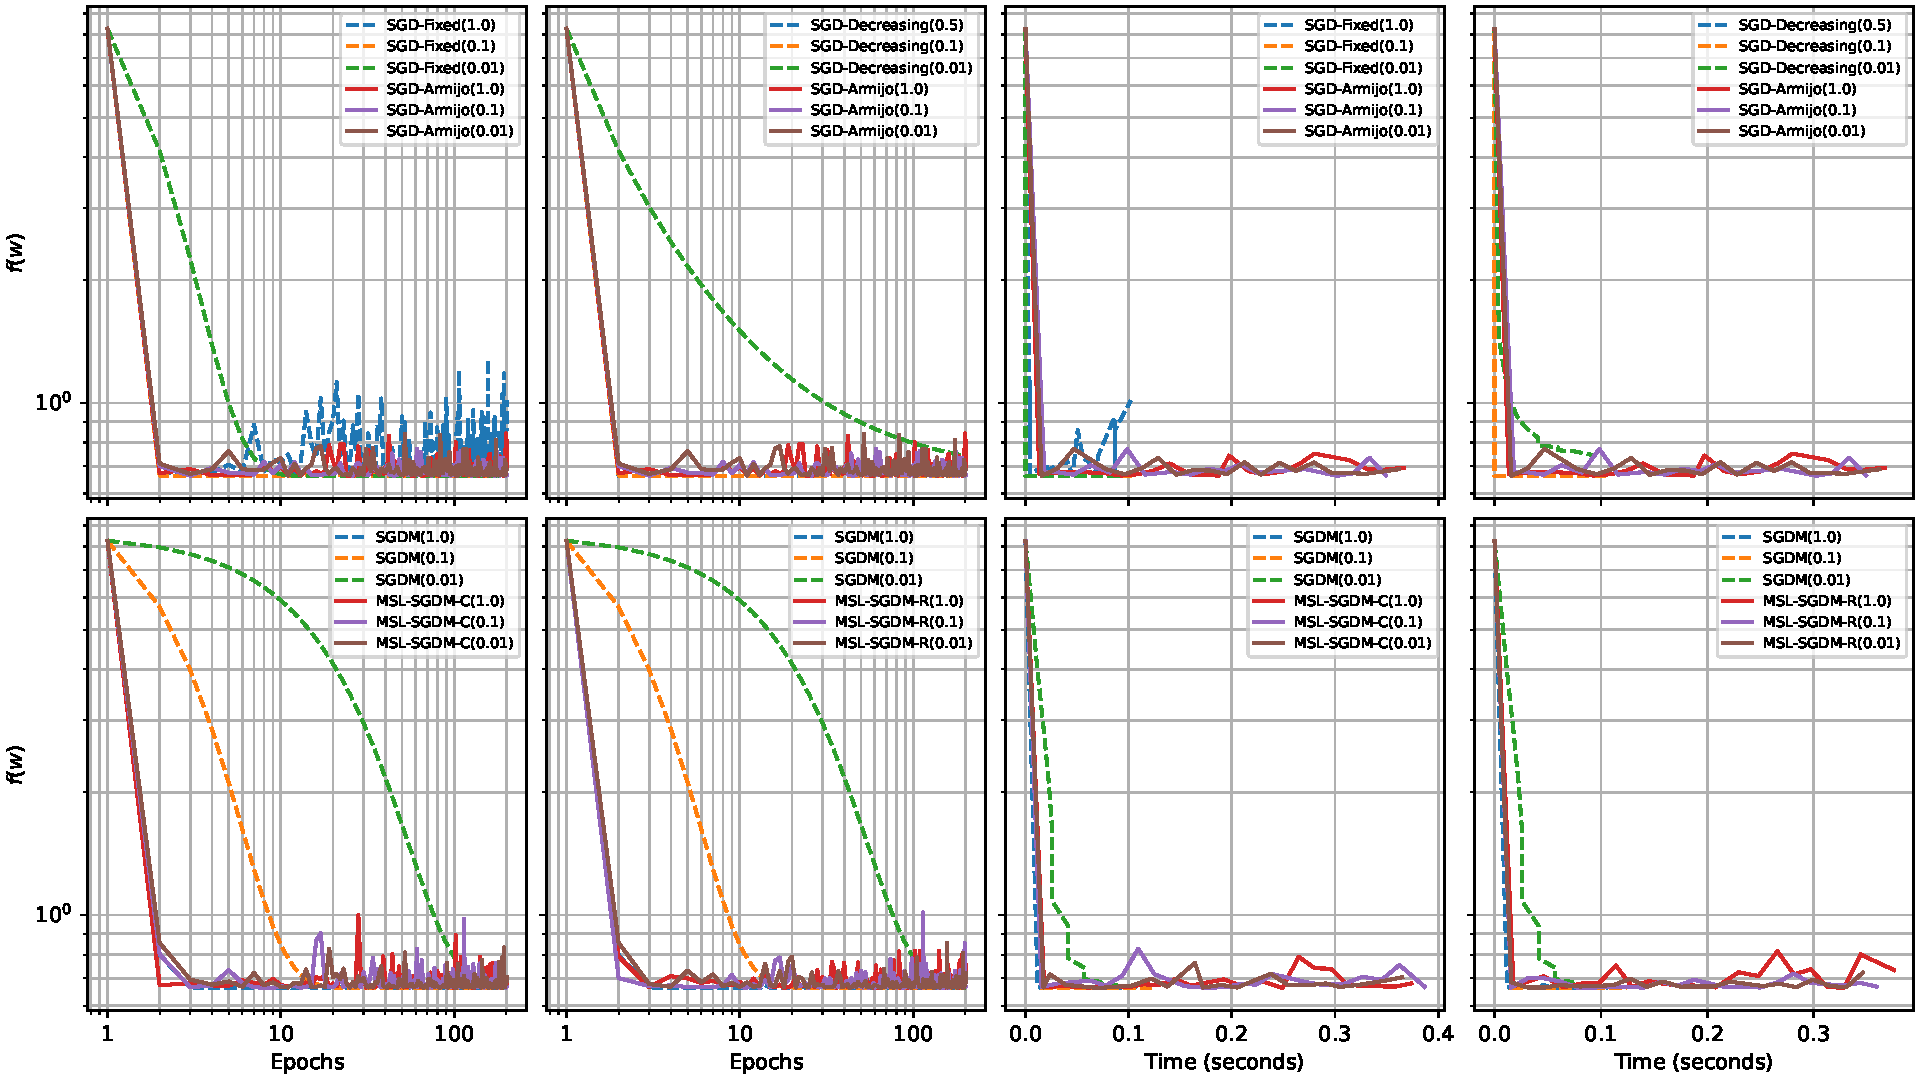
\includegraphics[width=\textwidth]{diab-diagnostic}} \\
% breast cancer
\subfloat[][\emph{Breast cancer dataset}\label{subfig:breast-diagnostic}]%
{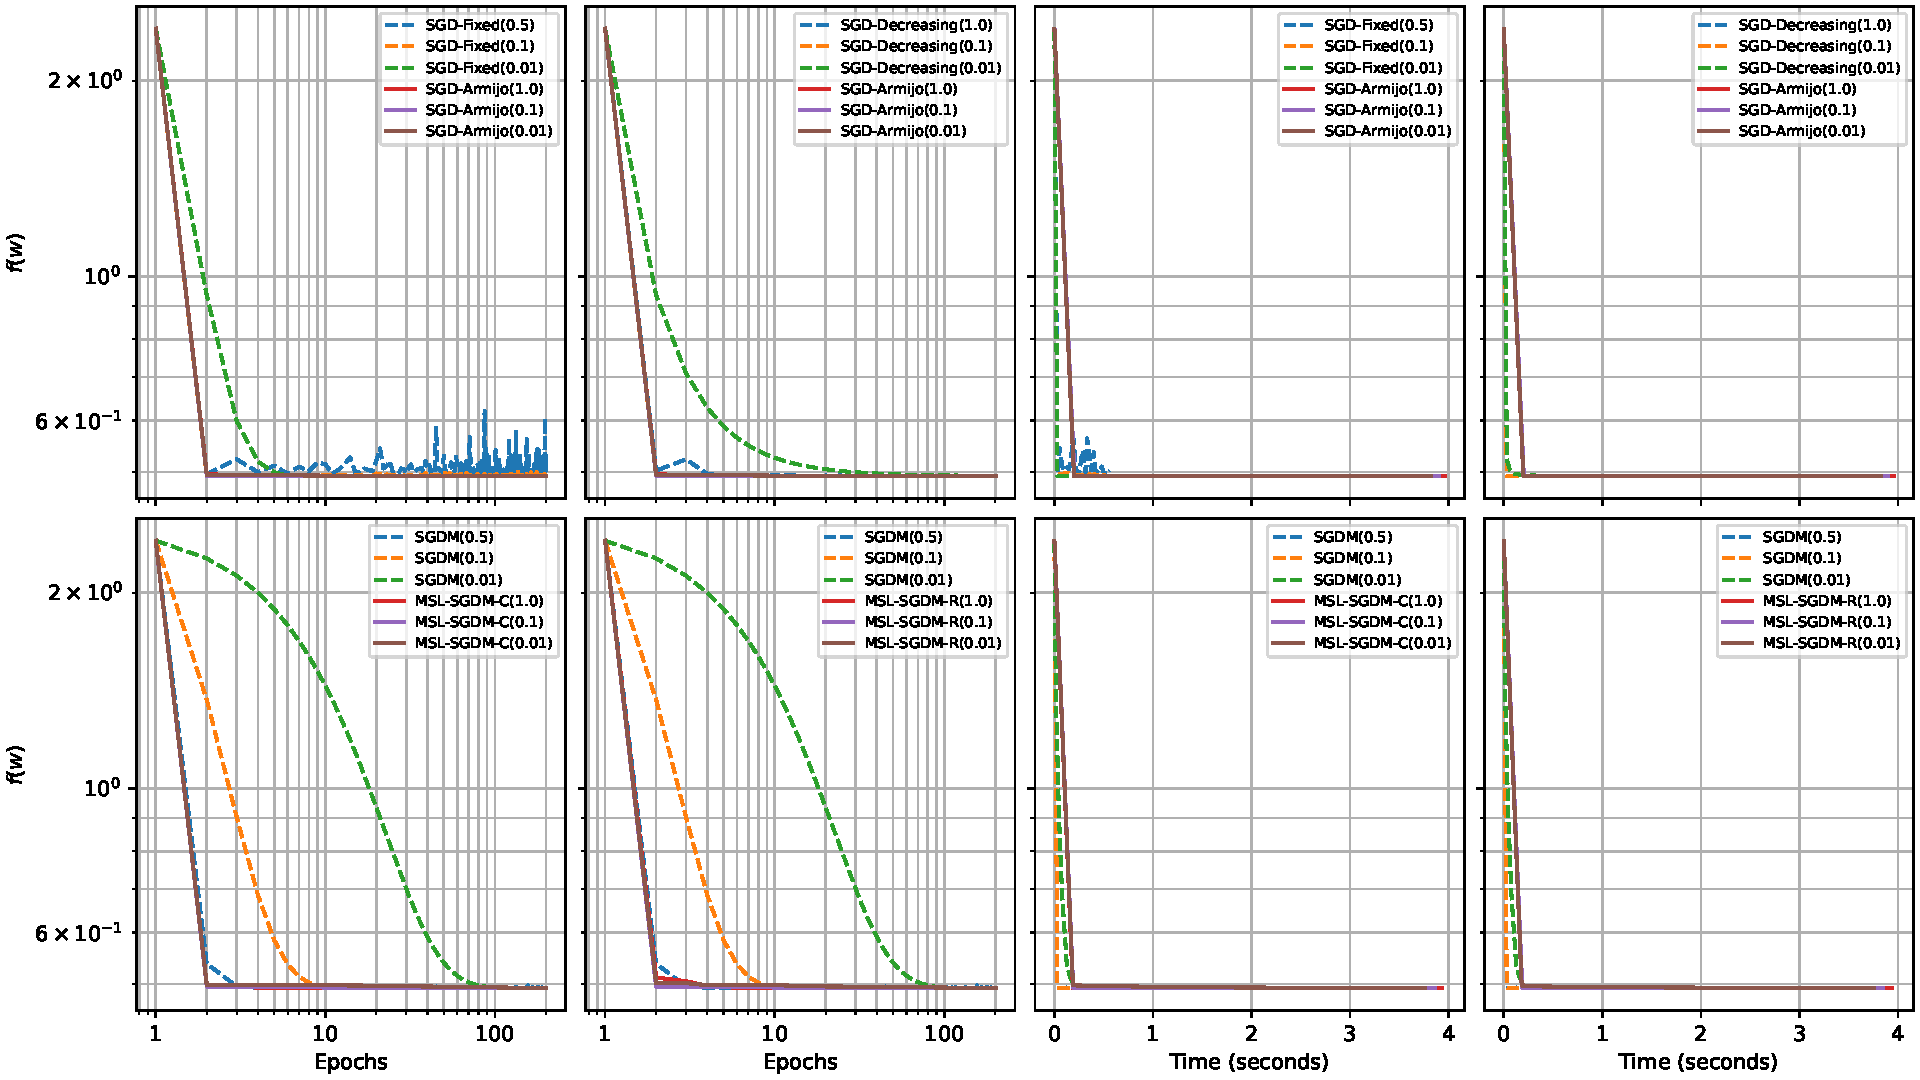
\includegraphics[width=\textwidth]{breast-diagnostic}} \\
\caption[]{Diabetes and Breast cancer}
\label{fig:diab-breast}
\end{figure}

\begin{figure}
\centering
% svmguide1
\subfloat[][\emph{svmguide1 dataset}\label{subfig:svm-diagnostic}]%
{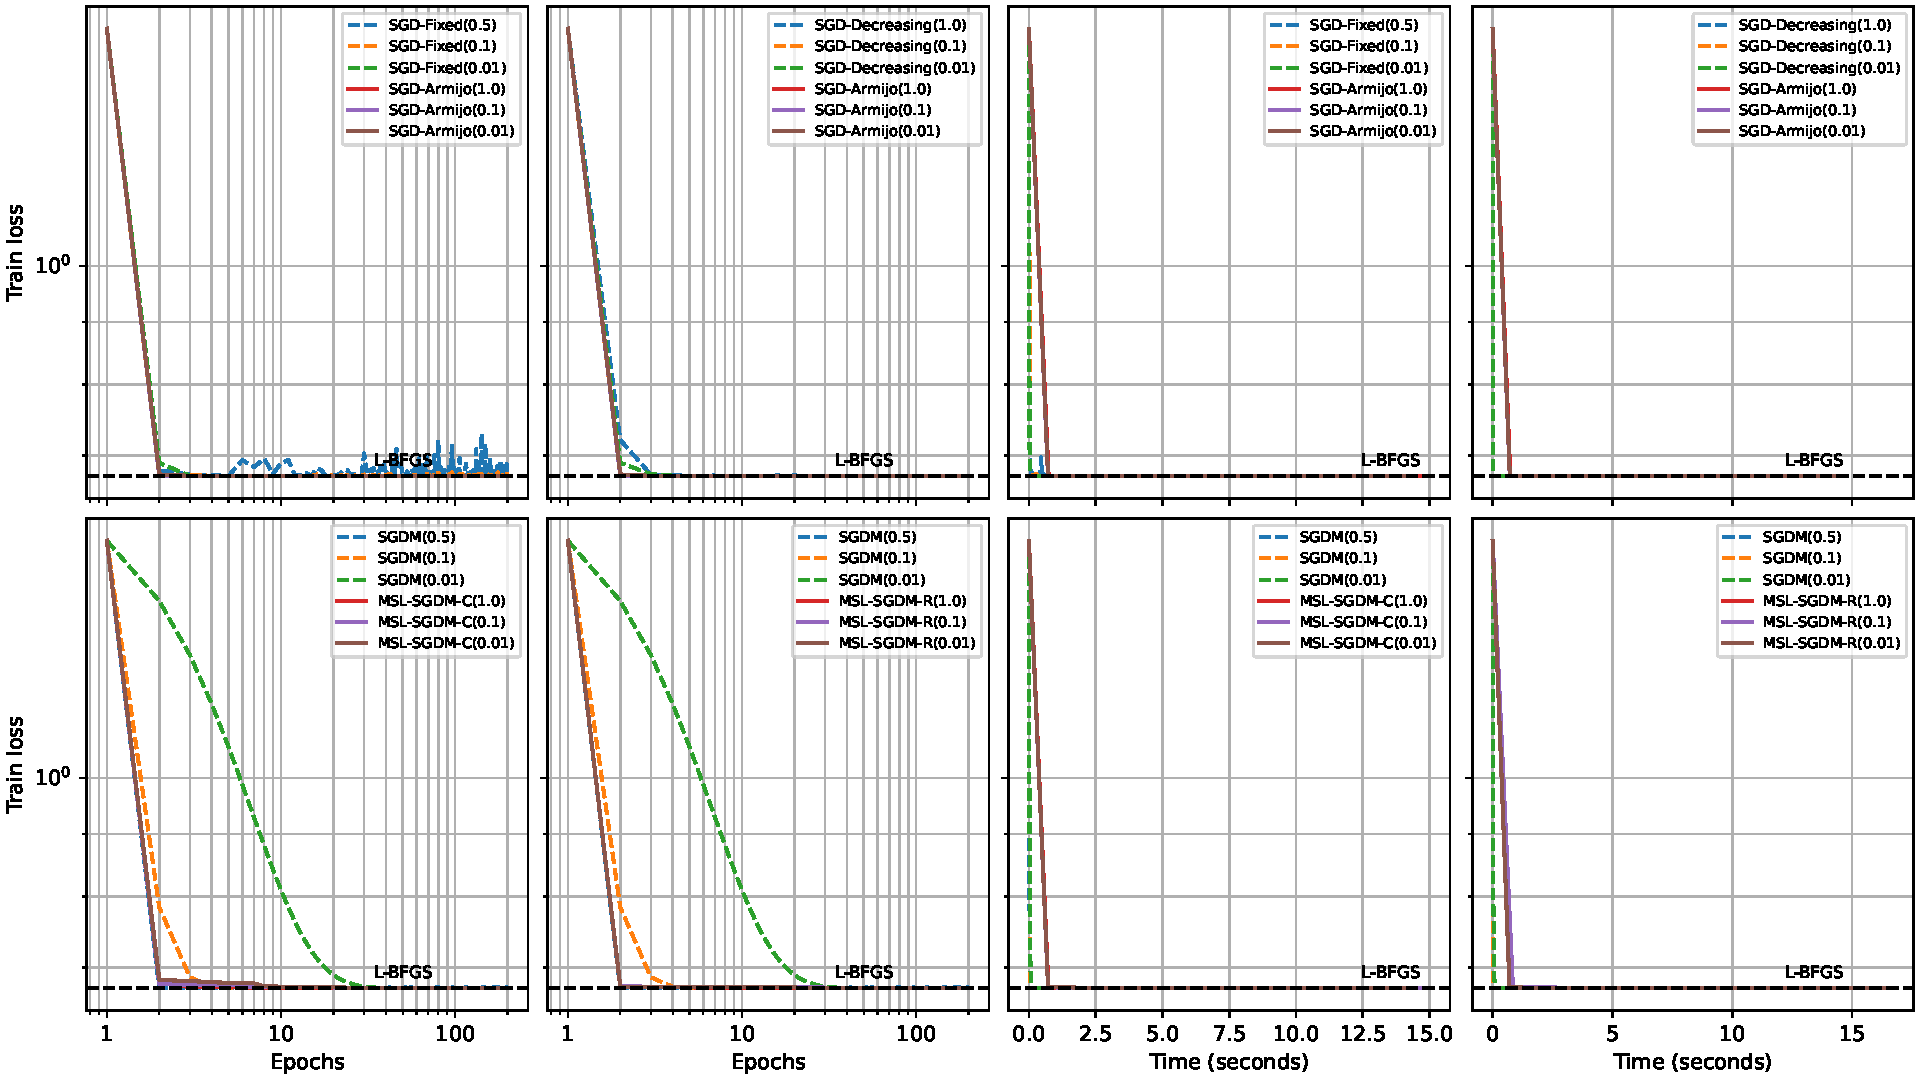
\includegraphics[width=\textwidth]{svm-diagnostic}} \\
% australian
\subfloat[][\emph{Australian dataset}\label{subfig:austr-diagnostic}]%
{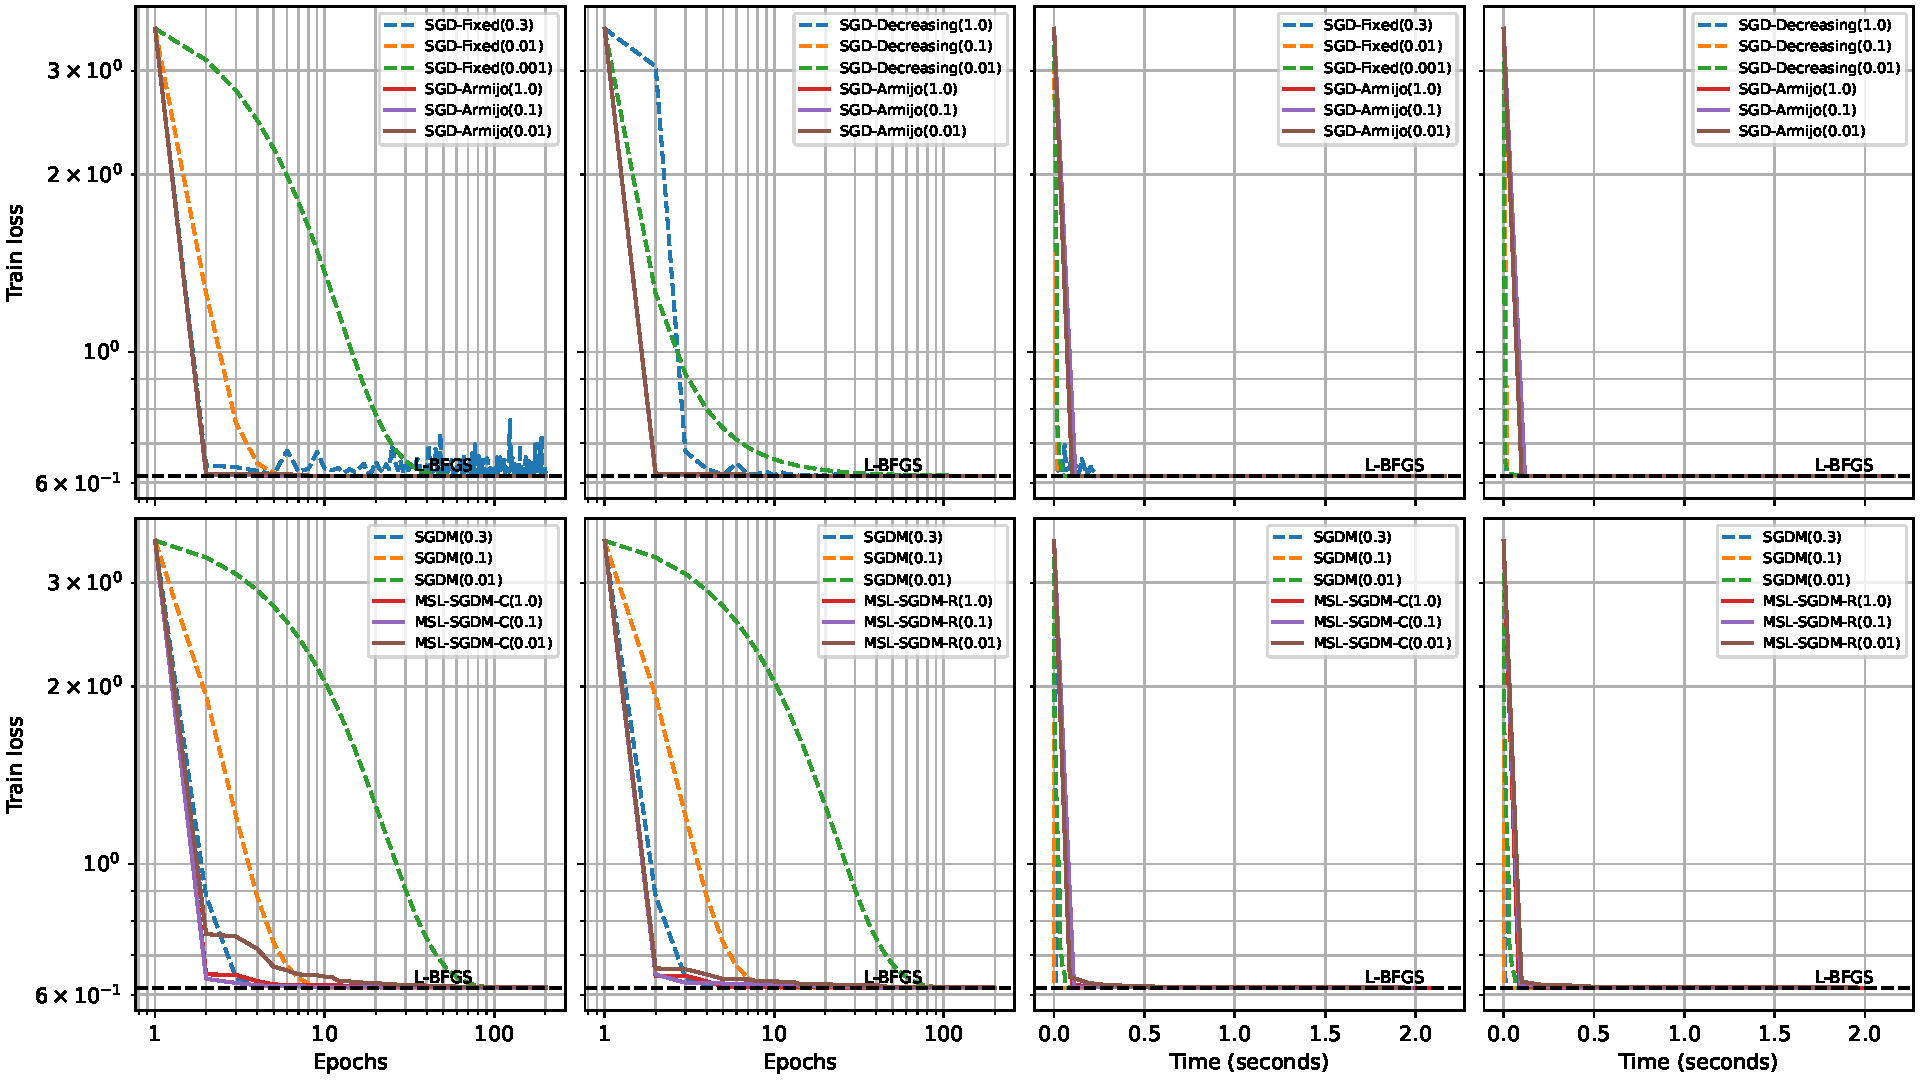
\includegraphics[width=\textwidth]{austr-diagnostic}}
\caption[]{svmguide1 and Australian datasets}
\label{fig:svm-austr}
\end{figure}

\begin{figure}
\centering
% mushrooms
\subfloat[][\emph{Mushrooms dataset}\label{subfig:mush-diagnostic}]%
{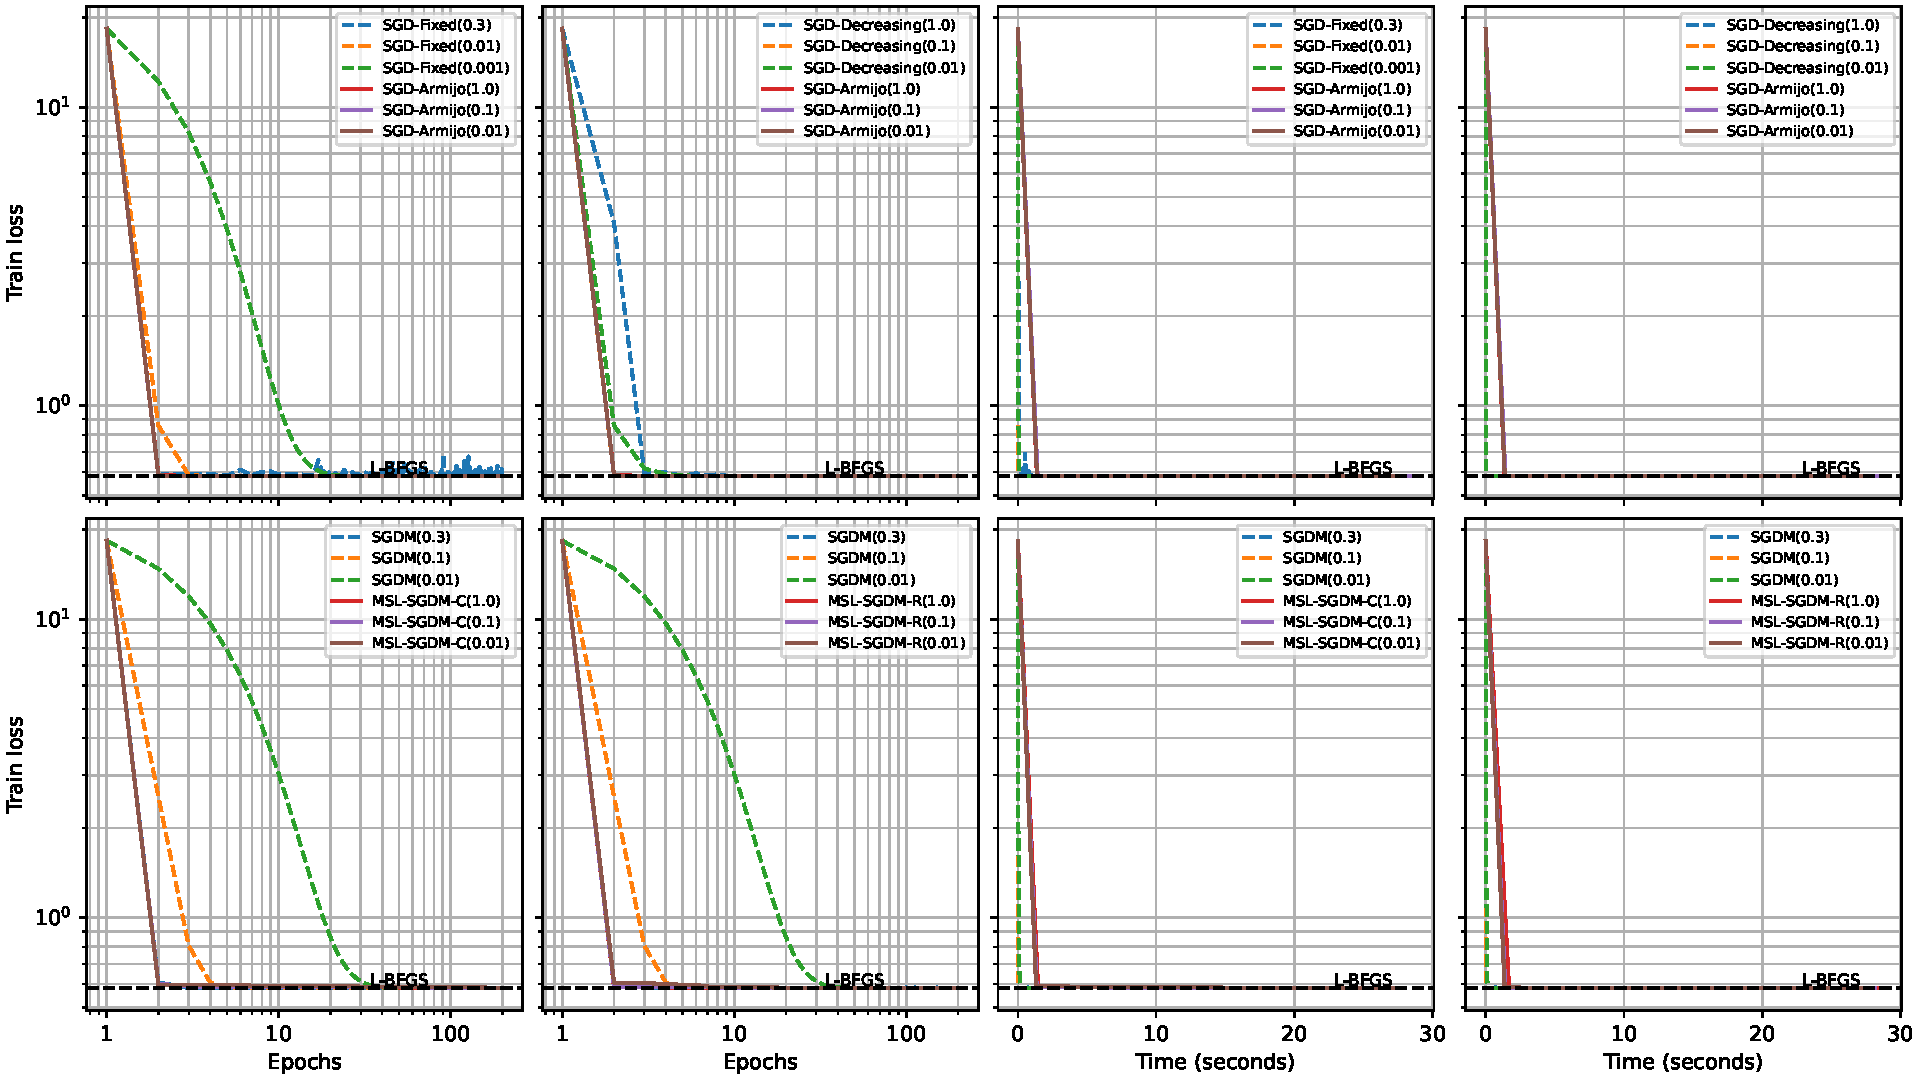
\includegraphics[width=\textwidth]{mush-diagnostic}} \\
% german
\subfloat[][\emph{German dataset}\label{subfig:german-diagnostic}]%
{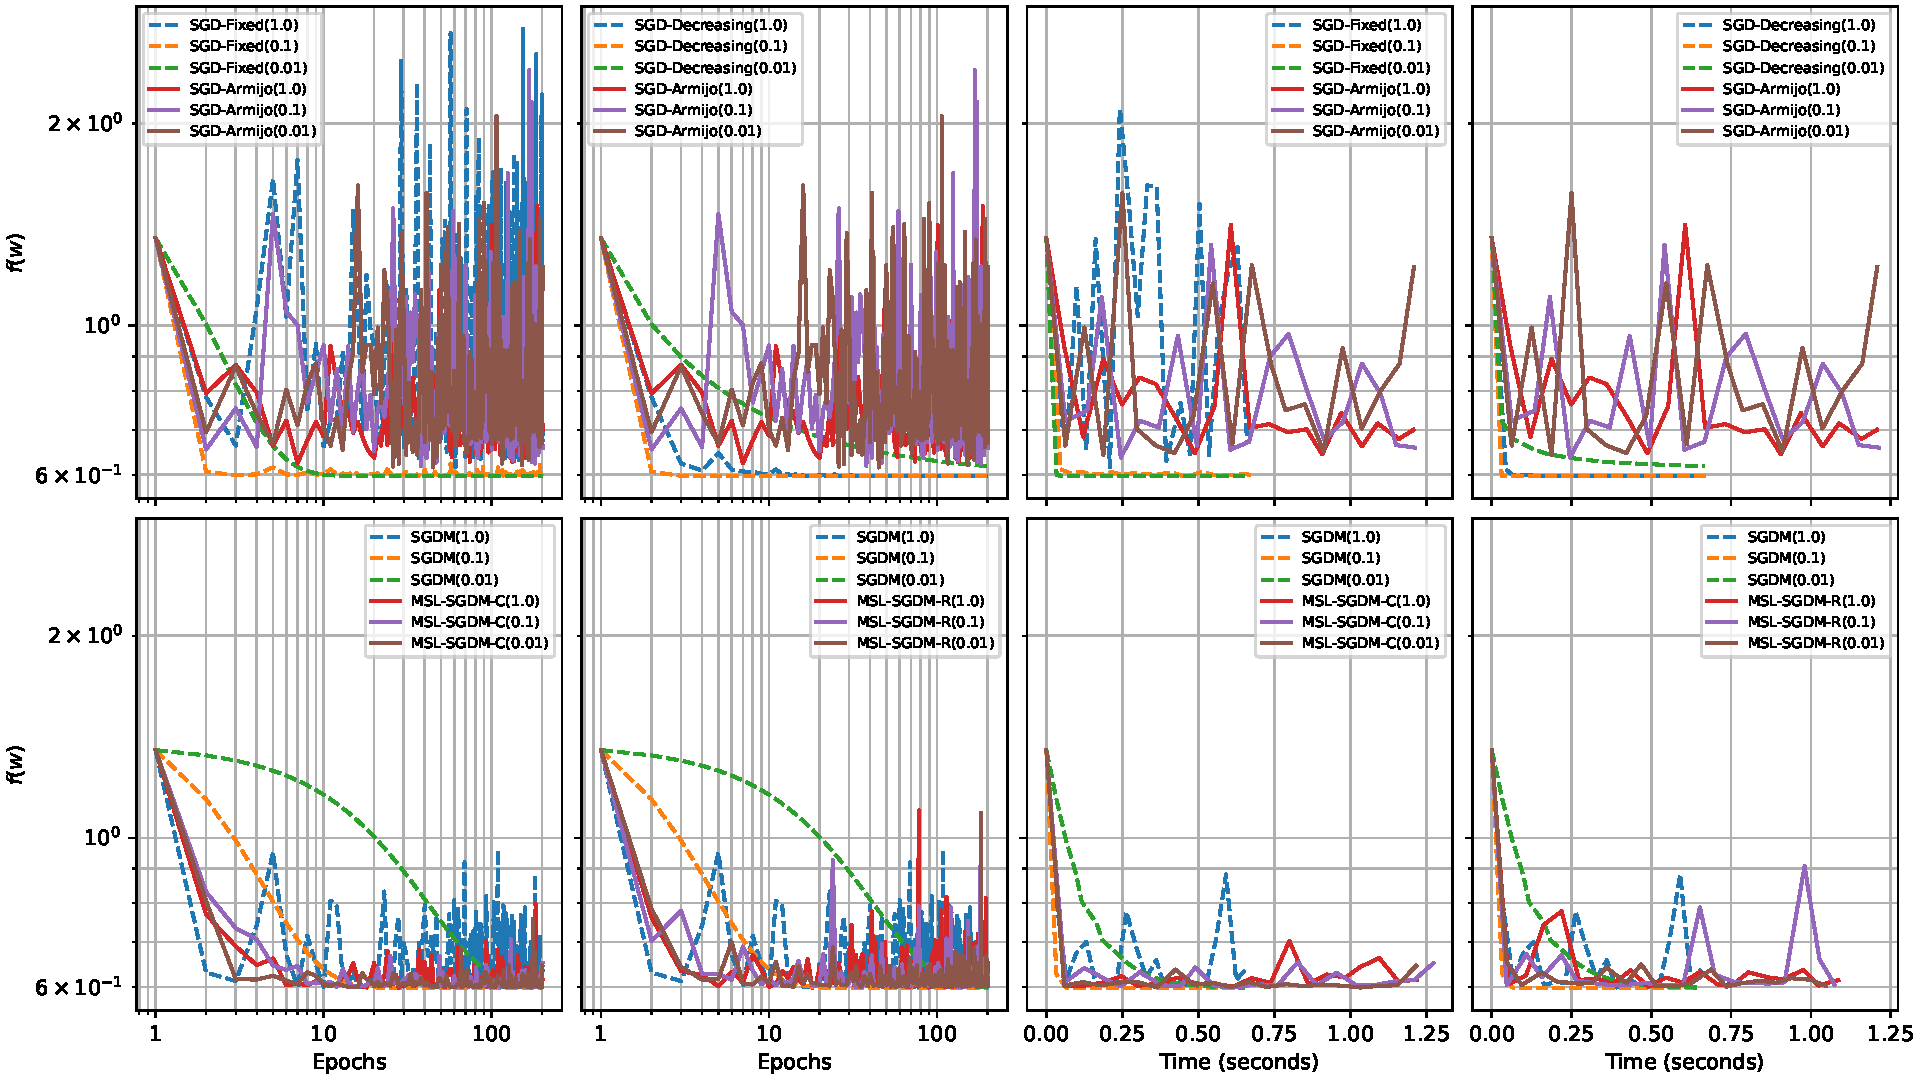
\includegraphics[width=\textwidth]{german-diagnostic}}
\caption[]{Mushrooms and German datasets}
\label{fig:mush-german}
\end{figure}

%\cleardoublepage
% ***************************************************** %
%\section{Mathematical background}
% ***************************************************** %

%\begin{defs}[Convex function]\label{def:conv_fun}
%	Let $S\subseteq\R^n$ be a convex set, a function $f\colon S\to\R$ is said to be convex if the hessian matrix is semi-positive-defined. If the hessian matrix is positive-defined, then the function is strictly convex.
%\end{defs}
%
%\begin{thm}[Weirstrass theorem]\label{thm:weirs}
%	Let $f\colon\R^n\to\R$ be a continuous function and $S\subseteq\R^n$ a compact set. Then function $f$ admits global minimum in $S$.
%\end{thm}
%
%\begin{cor}[Sufficient condition]\label{cor:weirs1}
%	If function $f\colon\R^n\to\R$ is a continuous and coercive function, then $f$ admits global minimum in $\R^n$.
%\end{cor}
%
%\begin{prop}[Coercivity of a quadratic function]
%	A quadratic function $\func(x)=\frac{1}{2}x^TQx-c^Tx$ is said to be coercive if and only if the symmetric matrix $Q\in\R^{n\times n}$ is positive-defined.
%\end{prop}
%
%\begin{prop}[Unique global minimum]\label{prop:min_unique}
%	Let $S\subseteq\R^n$ be a convex set, let $f\colon S\to\R$ be a strictly convex function. Then the global minimum, if exists, is unique.
%\end{prop}
%
%\begin{prop}[First order optimality condition]
%	$\bar{x}$ is a local minimum for $f\colon\R^n\to\R$ of class $f\in C^1(\R^n)$ if and only if $\nabla\func(\bar{x})=0$.
%\end{prop}
%
%\begin{prop}[Second order optimality condition]\label{prop:opt_second}
%	$\bar{x}\in\R^n$ is a local minimum for $f\colon\R^n\to\R$ of class $f\in C^2(\R^n)$ if and only if
%	\[\nabla\func(\bar{x})=0\quad\wedge\quad \nabla^2\func(\bar{x})\,\,\,\text{positive semi-definite}\]
%\end{prop}

% add definition of coercive function and proposition about compact sets?
% add gradient descent?
